%
% Chapter 5
%

\chapter{Event Reconstruction}
\label{event_reco}

The particle flow (PF) event reconstruction aims to reconstruct and identify each particle in an event with an optimized combination of information from the various CMS detector elements~\cite{Sirunyan:2017ulk}. In this process, identifying the PF candidate type (photon, electron, muon, charged, and neutral hadrons) plays a vital role in determining particle direction and energy. The PF algorithm links several PF elements that a physics object can give rise to across different sub-detector layers. The PF elements are tested for their compatibility in the $\eta$--$\phi$ plane and are combined to form PF blocks. A predefined sequence of reconstruction and identification algorithms are run in each of these PF blocks. This sequence starts with the reconstruction and identification of muon candidates. PF quality criteria are placed for the muon candidate. The PF elements associated with a muon candidate passing these criteria are removed from the block. The next step in the sequence is to reconstruct and identify electron candidates. The electrons are defined as PF electrons if the tracker's extrapolated tracks have a corresponding energy deposit in the ECAL. The sequence now proceeds with identifying photons and hadrons. In the sequence, tracks with momentum uncertainty more than the calorimeters' resolution are removed to reduce fake track identification. All the remaining tracks are associated with charged hadrons, and all the remaining calorimeter energy deposits are associated with photons (ECAL) and hadrons (HCAL). At the end of this sequence, we are left with a list of all electrons, photons, muons, charged hadrons, and neutral hadrons in the event with optimally determined direction, charge, and energy.


\section{Track and primary vertex reconstruction}

The hits from the pixel and strip detectors in the tracker are used to reconstruct the tracks of charged particles~\cite{Chatrchyan:2014fea}. Signals above specified thresholds in the pixel and strip channels are clustered to form the hits. The cluster positions and corresponding uncertainties are estimated in a local orthogonal system plane of each sensor. A translation is done between the local coordinate system of these hits to the tracks' global coordinate system during track reconstruction. Kalman filter (KF)~\cite{Fruhwirth:1987fm} based algorithm is used to reconstruct tracks and is called the combinatorial track finder. Tracks with high \pt and those produced near the interaction region are easiest to find. Track reconstruction uses an iterative procedure with the initial iterations searching for the most accessible tracks. In subsequent iterations, tracks with low \pt and those produced far from the interaction region are searched. Hits unambiguously assigned to the track in the previous iterations are removed. This reduces the combinatorial complexity in the subsequent iterations. In each iteration, there are four sequential steps.

The first step in the sequence is seed generation. The magnetic field causes the charged particles to follow a helical path, requiring five parameters to determine the trajectory. These parameters are extracted using two or three hits in the inner region of the tracker. The seeds are constructed in the inner part owing to the high granularity of the pixel detectors. The tracks are then constructed outwards. The motivation to use the inner region for seed construction also rests on the fact that particles like pions and electrons interact inelastically with tracker material as they traverse through the tracker to its outer regions.

KF based algorithm is then used for track finding. Track parameters are estimated by using the trajectory seeds generated in the previous step. The seed trajectories are extrapolated along the expected path of a charged particle. The track candidates are built using the location and uncertainty of detected hits, taking into account effects such as Coulomb scattering at successive detector layers. The parameters are updated at each layer. An analytical extrapolation is done that determines which adjacent layers of the detector the trajectory can intersect. A search is performed for silicon modules in these layers that are compatible with the extrapolated trajectory. Mutually exclusive groups are built from all compatible modules in each layer such that no two modules in each group overlap. One of the compatible hits from a group of hits is added to the original track candidate to form new track candidate. The added hits' information is combined with the original track candidates' extrapolated trajectory to update the new candidates' trajectory parameters. Figure~\ref{fig:trackeff} illustrates the reconstruction efficiency of tracks in the case of isolated muons.

The hits from the last step are refitted using a KF in a phase called track fitting. This provides the best possible estimate of parameters for each track trajectory. There can be several fake tracks that are not associated with any charged particle passing through the tracker. Several quality requirements are applied to the set of reconstructed tracks, which substantially reduces the fake contribution. The quality criterion involves the minimum number of layers the track has hits in, how compatible its origin is with a primary vertex (PV), and how good a fit it yields.

The interaction vertices in the \pp collisions are reconstructed by selecting tracks produced promptly in the primary interaction region. The chosen tracks are clustered based on their z-coordinates at their closest approach to the beam spot center. The beam spot represents a 3-D profile of the region where the proton beams collide inside the CMS detector. The adaptive vertex fitter procedure is used for finding the exact positions of the vertices from these clustered candidates~\cite{Fruhwirth:2007hz}. The PV has the most significant sum of squared transverse momenta of tracks originating from it.

\begin{figure*}[!htpb]
  \centering
  \captionsetup{width=0.98\textwidth,justification=centering}
  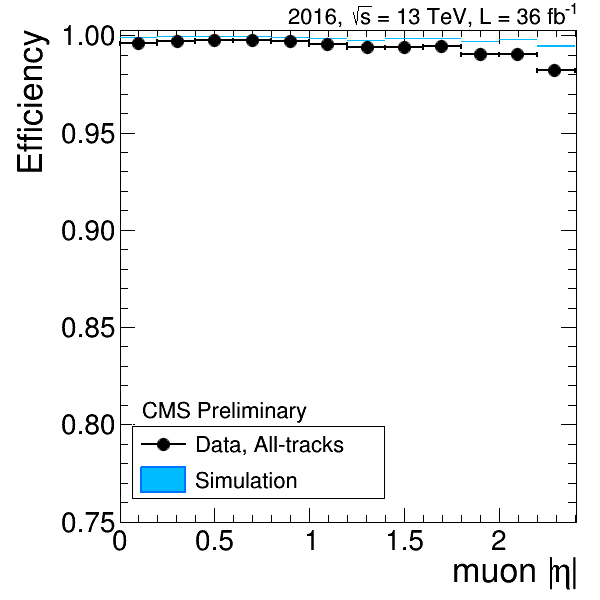
\includegraphics[width=0.45\textwidth]{plots/chapter5/TrackEta2016.png}
  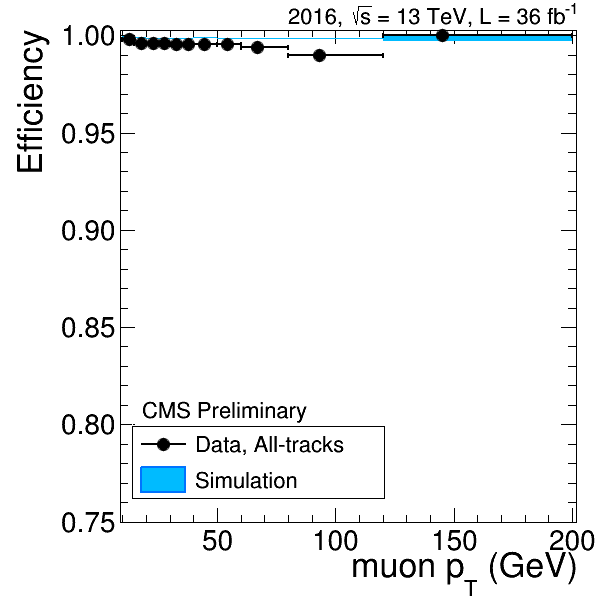
\includegraphics[width=0.45\textwidth]{plots/chapter5/TrackPt2016.png} \\
  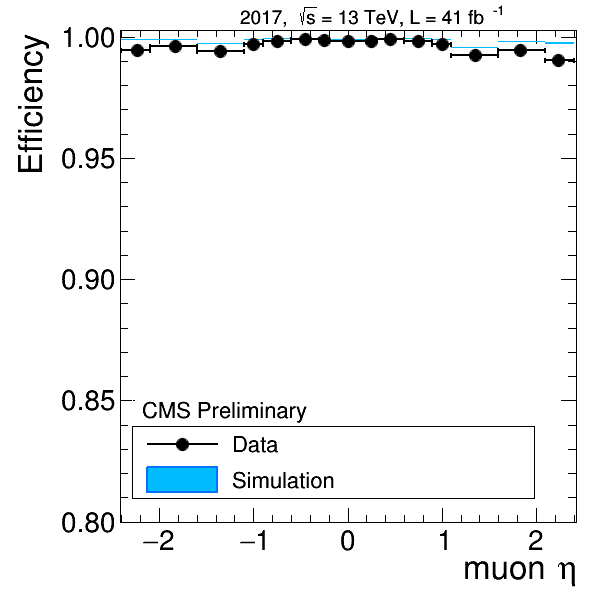
\includegraphics[width=0.45\textwidth]{plots/chapter5/TrackEta2017.png}
  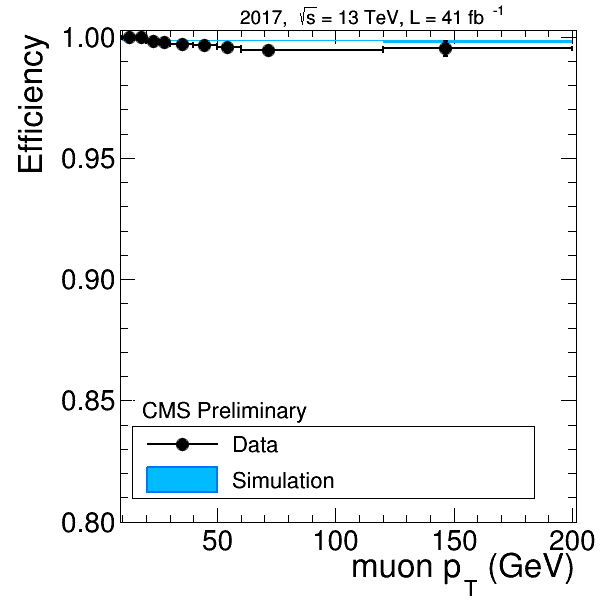
\includegraphics[width=0.45\textwidth]{plots/chapter5/TrackPt2017.png} \\
  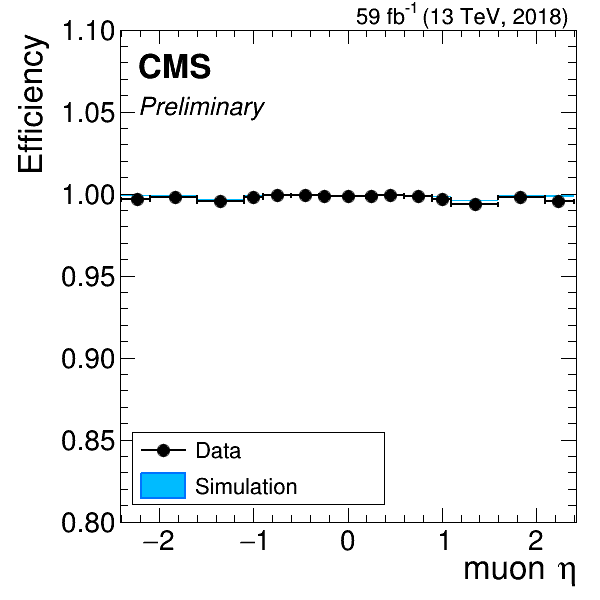
\includegraphics[width=0.45\textwidth]{plots/chapter5/TrackEta2018.png}
  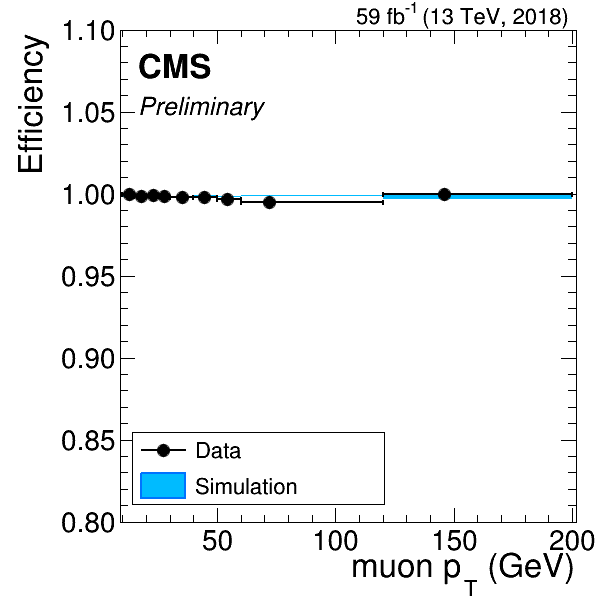
\includegraphics[width=0.45\textwidth]{plots/chapter5/TrackPt2018.png} \\
  \caption{The tracking efficiency for ``all-tracks'' collection as a function of pseudorapidity and transverse momentum for muons coming from the \PZ decay.}
  \label{fig:trackeff}
\end{figure*}


\section{Muon reconstruction}

Muons are reconstructed using the hits in the muon system, and tracks from the tracker~\cite{Sirunyan:2018fpa}. The gas in the muon chambers is ionized when muons traverse through them. The ionization is read-out by electronics systems that associate these ``hits'' with well defined locations in the detector. The hits in the muon chambers are reconstructed independently of track reconstruction in the tracker. KF is used for reconstructing the hits from the muon system. These tracks are called standalone-muon tracks. Tracker tracks with $\pt > 0.5 \GeV$ are propagated to the muon system. Muon tracks are built from these tracks by matching them to segments of hits in DT or CSC. A matching tracker track is called a tracker muon track. Standalone-muon tracks can be matched with tracker tracks and combining information from both using a KF fit. The muon tracks built in such a manner are called global muon tracks. Muons leaving hits in several muon stations have a very efficient global muon reconstruction. Muon candidates with low \pt have an efficient tracker muon reconstruction. However, it can cause fake muon tracks due to hadronic particles, which punch-through to the innermost muon stations. The global muon reconstruction reduces the muon misidentification rate compared to tracker muons. The efficiency for reconstructing a muon is as high as 99\% when tracker muon tracks and global muon tracks are combined. PF algorithm applies the quality criterion for the reconstructed muon candidates. The PF muon candidates used in the analysis were required to satisfy the following set of criterion to be identified as a muon:

\begin{itemize}
  \item The candidate is reconstructed as a global muon along with PF muon identification.
  \item $\chi^{2}$/ndof of the global muon track fit $< 10$.
  \item At least one muon chamber hit included in the global muon track fit.
  \item There should be muon segments in at least two muon stations. This implies that the muon is also an arbitrated tracker muon.
  \item Its tracker track has transverse impact parameter $|\text{dxy}| < 2~\mm$ with respect to the PV.
  \item The longitudinal distance of the tracker track with respect to the PV is $|\text{dz}| < 5~\mm$.
  \item Number of pixel hits $> 0$.
  \item Number of tracker layers with hits $> 5$.
\end{itemize}

PF muon identification efficiency is illustrated using a plot from a study performed by the CMS muon physics object group in Figure~\ref{fig:muoneff}. There are differences in the efficiencies in data and MC simulation. They are corrected using a set of scale-factors applied as a function $\eta$ and \pt to adjust the simulation efficiency to match the efficiency in data.

\begin{figure*}[!htpb]
  \centering
  \captionsetup{width=0.98\textwidth,justification=centering}
  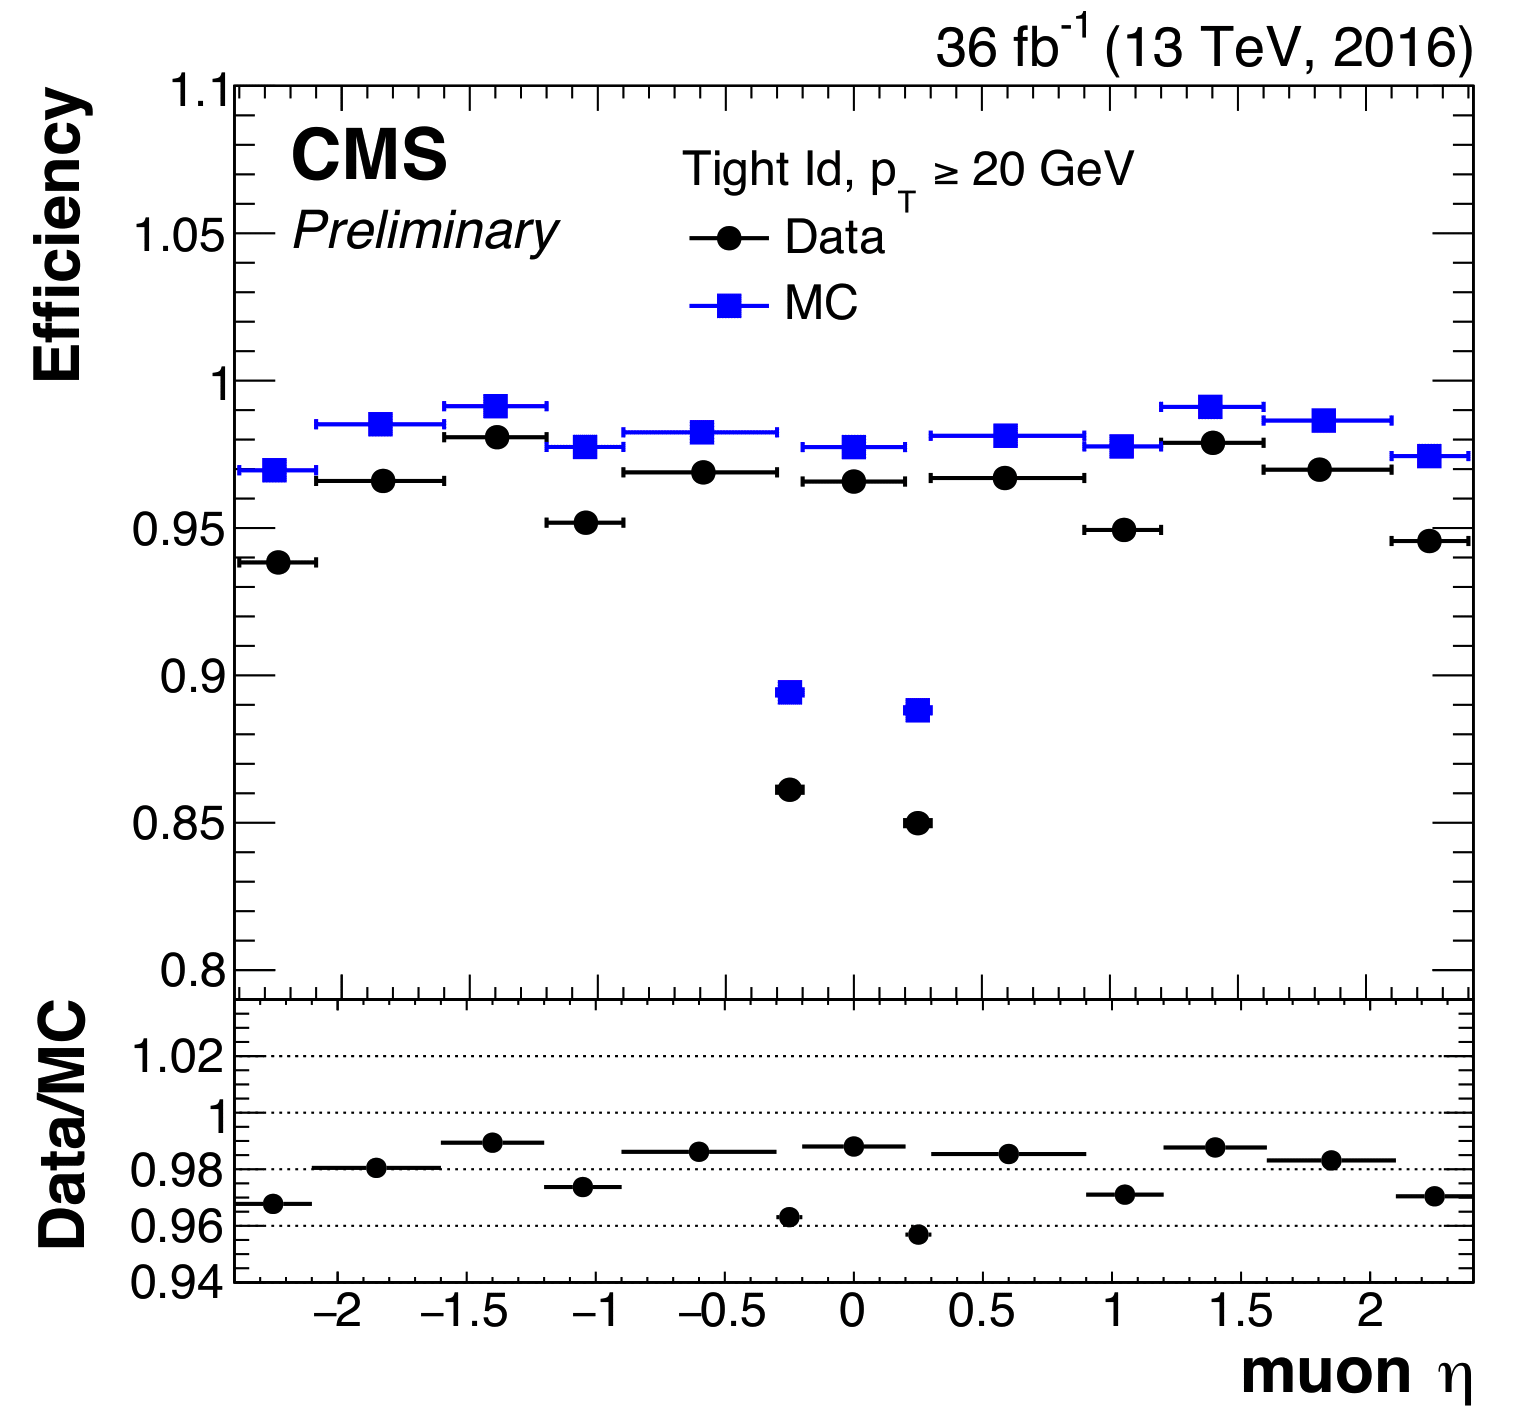
\includegraphics[width=0.49\textwidth]{plots/chapter5/Eta2016.png}
  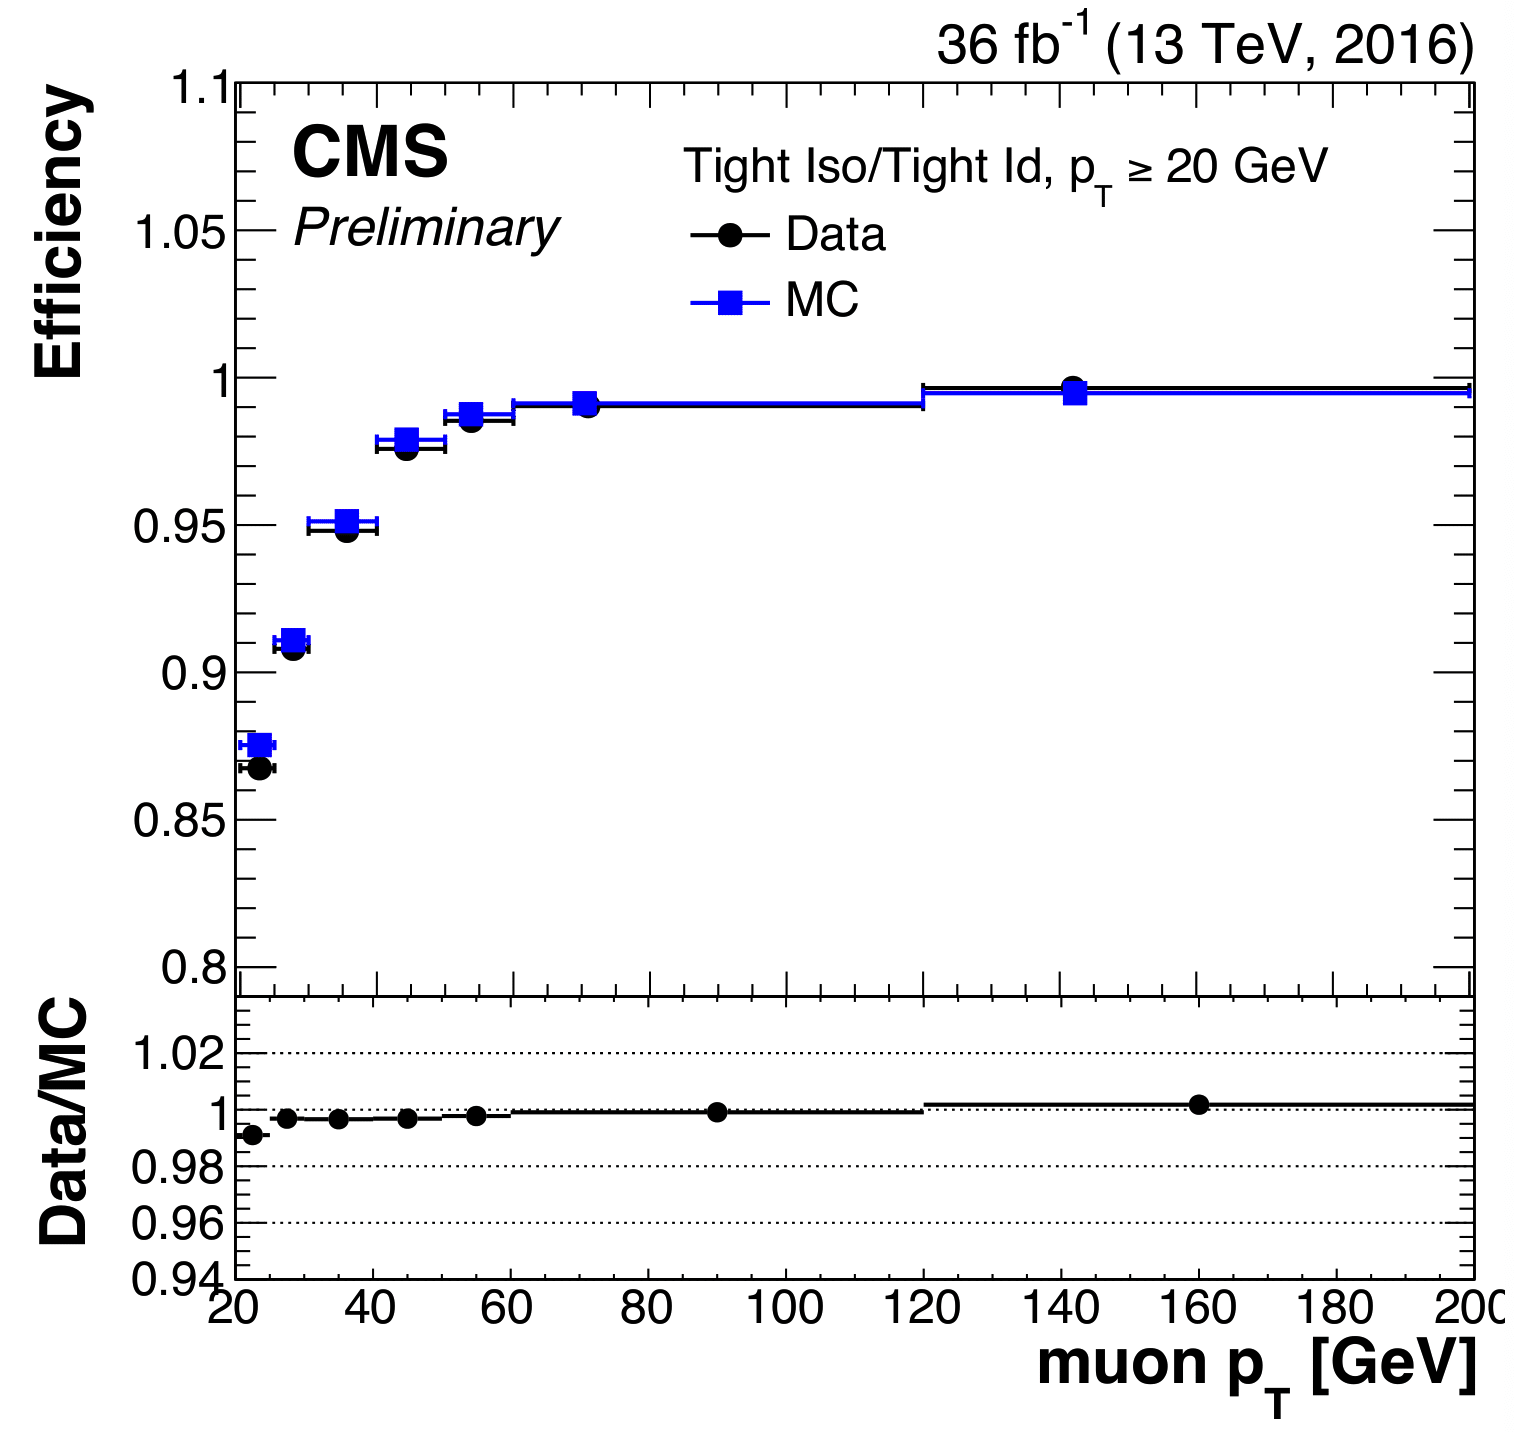
\includegraphics[width=0.49\textwidth]{plots/chapter5/Pt2016.png} \\
  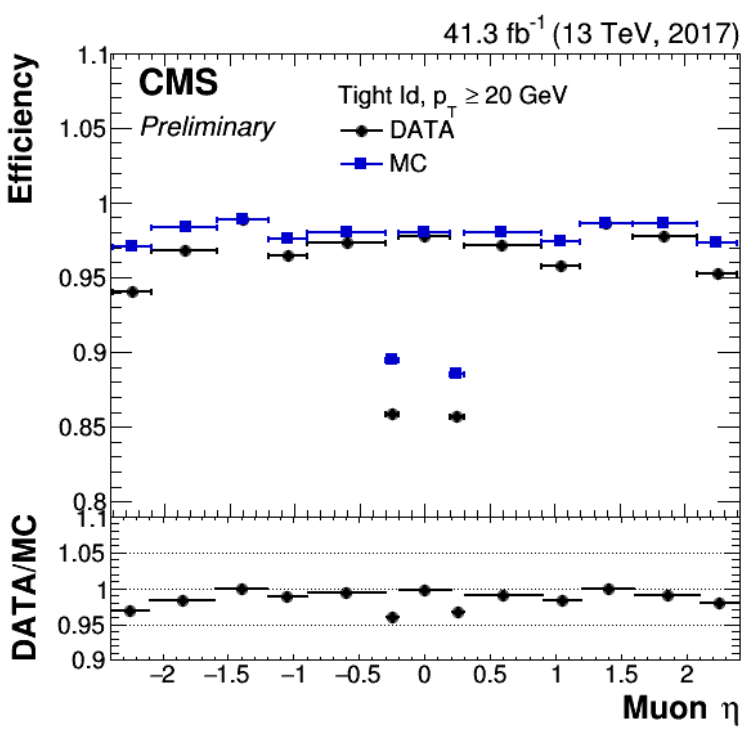
\includegraphics[width=0.49\textwidth]{plots/chapter5/Eta2017.png}
  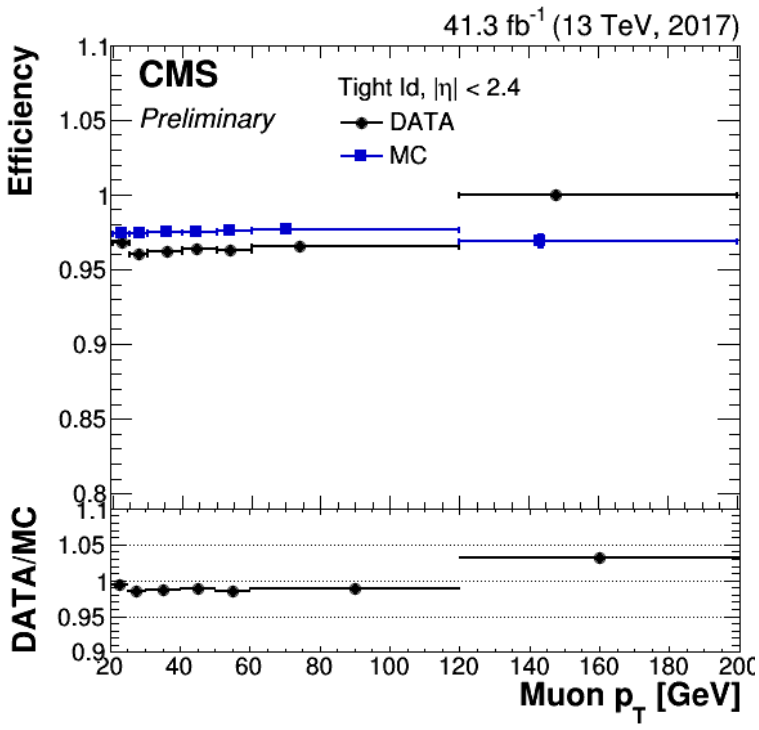
\includegraphics[width=0.49\textwidth]{plots/chapter5/Pt2017.png} \\
  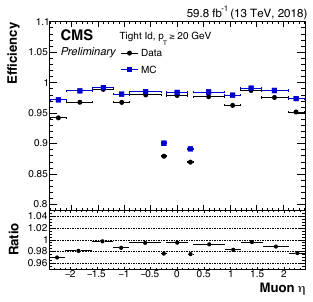
\includegraphics[width=0.49\textwidth]{plots/chapter5/Eta2018.png}
  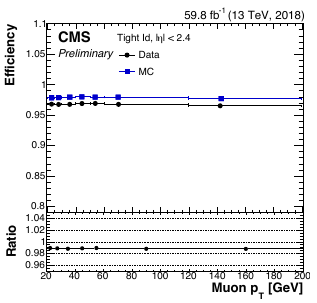
\includegraphics[width=0.49\textwidth]{plots/chapter5/Pt2018.png} \\
  \caption{Efficiency of muon identification as a function of $\eta$ and \pt, for data (black) and simulation (blue)~\cite{muon_pog}.}
  \label{fig:muoneff}
\end{figure*}


\section{Electron reconstruction}

Clusters of energy formed in the ECAL are associated with tracks from the tracker to reconstruct electrons. Electrons radiate bremsstrahlung photons caused by the interaction of electrons with atoms as they pass through the tracker. The radiation depends on the amount of detector material the electron has to cross. The clustering algorithm needs to account for these bremsstrahlung photon showers' energy to measure the electron's energy. The bremsstrahlung photons' energy spreads primarily in the $\phi$ direction, and the spread in the $\eta$ direction is relatively small.

The hybrid algorithm is used to cluster the electron energy deposit in the ECAL barrel. It uses the geometry of the ECAL to form clusters that are wide in the $\phi$ direction but are narrow in the $\eta$ direction. A seed crystal contains the most significant energy deposited in the considered region above a 1~\GeV threshold. A $5 \times 1$ array of crystals are added in $\eta\times\phi$ around the seed crystals in both directions of $\phi$ if the energy contained in the array is above the 0.1~\GeV threshold. Contiguous arrays are merged into clusters. An electron supercluster is formed from all such strip clusters, which have at least one seed strip with energy above the 0.35~\GeV threshold. A different clustering algorithm is used in the ECAL endcap due to the crystals' different geometrical arrangements. This algorithm is called the $5 \times 5$ algorithm. It starts with a seed crystal satisfying the minimum energy requirement of 0.18~\GeV. A supercluster is formed by progressively grouping clusters of $5 \times 5$ crystals around the seed crystal. The added clusters need to have energy over 1~\GeV and be within $\pm 0.7$  and $\pm 0.3$ respectively in $\eta$ and $\phi$ around the seed crystal. The energy-weighted mean of the cluster positions is taken as the position of the supercluster. The sum of the energy of all its constituent clusters is its energy. The energy from the preshower is also added to the supercluster. This is implemented by using it's most energetic cluster and it's maximum distance in $\phi$ to other clusters and extrapolating it to the preshower plane to define the spread in the preshower.

A dedicated tracking procedure is used for electron candidates that use information from the tracker and the ECAL. The first step in electron track reconstruction is seeding. The reconstructed superclusters' position and energy can constrain the trajectory of the electron through the tracker and the assumption that the electrons originated close to the center of the beam spot. The electron seeds are the hits in the first layers of the trackers compatible with these trajectories. In an alternative approach, tracks constructed by the standard tracking algorithm are extrapolated to the ECAL and matched with a supercluster. The seed collections from these two approaches are merged, leading to an increase in the seeding procedure's overall efficiency. Electron track finding and fitting phases use these seeds. The track finding procedure is adjusted to accommodate tracks that deviate from their expected trajectory because of bremsstrahlung. The penalties assigned to track candidates for passing through a tracker layer without being assigned a hit are similarly adjusted. The Gaussian sum filter (GSF) is used for the final track fit. This accounts for the fact that the energy loss of an electron traversing the tracker material is non-Gaussian. As the KF algorithm assumes Gaussian distribution, the GSF technique deals with this by approximating this non-Gaussian energy loss distribution as the sum of several Gaussian functions and performs much better than the regular fitting procedure.

The electron candidates are constructed by associating the GSF track produced by the above procedure with a supercluster in the ECAL. A geometrical matching in $\eta$--$\phi$ is used for the association for ECAL seeded candidates. A multivariate (MVA) technique that combines information from supercluster and GSF track is used for tracker seeded candidates. The electron's charge is estimated using the GSF track curvature, ECAL supercluster's relative position in $\phi$ to that of the first hit in the GSF track, and KF tracks that have common hits with the GSF tracks. This combined approach reduces the charge misidentification probability to 1.5\%. A combination of tracker and ECAL measurements is used for estimating the momentum of electrons.

Several quality criteria are placed on the reconstructed electron candidates to identify electrons. This helps in suppressing fake sources such as photon conversions, jets misidentified as electrons, etc. Electrons are required to pass an identification variable based on a boosted decision tree (BDT) discriminator, which uses track quality, shower shapes, and kinematic quantities. The following variables are used as input to the BDT:
\begin{itemize}
  \item Cluster shape variables $\sigma_{\ieta, \ieta}$ and $\sigma_{\iphi, \iphi}$, with \ieta and \iphi the integer label of the $\eta$ and $\phi$ of a calorimeter cell. The circularity 1 - $\frac{\text{E}_{1 \times 5}}{\text{E}_{5 \times 5}}$, with $\text{E}_{1 \times 5}$ and $\text{E}_{5 \times 5}$ the energies in a $1 \times 5$ and a $5 \times 5$ grid around the supercluster seed, respectively.
  \item Shape variable R9 = $\frac{\text{E}_{3 \times 3}}{\text{E}_{\text{SC}}}$, with $\text{E}_{3 \times 3}$ the energy in a $3 \times 3$ grid of cells around the supercluster seed and $\text{E}_{\text{SC}}$ the raw energy of the supercluster.
  \item The number of valid hits in the track fit, the $\chi^{2}$ of the track fit, and the $\chi^{2}$ of the GSF track fit.
  \item The number of GSF track hits, the number of expected missing inner hits, and the result of the conversion vertex fit.
  \item The distance $\Delta \eta$ and $\Delta \phi$ between the reconstructed supercluster and the associated track at the position of the PV, and the distance in $\eta$ between the supercluster and the track at the calorimeter surface.
  \item H/E, the ratio of the hadronic energy over the electromagnetic energy in the supercluster and E/P, the ratio of the supercluster energy over the momentum of the track associated with the electron.
  \item The ratio of the energy of the electron cluster and the momentum of the associated track, evaluated at the electron cluster, and $1/\text{E}_{\Pe} - 1/\text{P}_{\Pe}$, with $\text{E}_{\Pe}$ the energy of the electron candidate and $\text{P}_{\Pe}$ its momentum.
\end{itemize}

The BDT was trained on a \PZ/\Pgg MC sample generated with MadGraph5, in 3 $\eta$ bins for electrons with $\pt > 10 \GeV$. There are two versions of the MVA available for electron identification. The first one includes the electron isolation in training and another which does not include this, and their performance is illustrated in Figure~\ref{fig:elec_BDT}. This analysis uses the version without the isolation included in the training. An additional selection of electron isolation is used. This is done so that in the \ehad channel, the misidentified lepton background can be estimated using the isolation based sideband regions. Instead of using fixed cuts on the MVA score, the cuts are alternatively varied exponentially with \pt to achieve a more constant efficiency of 80\%. The electrons are also subject to the same impact parameter cuts as the muons: the impact parameters between the electron track (best track) and the PV are restricted as $|\text{dxy}| < 0.045$ cm and $|\text{dz}| < 0.2$ cm to ensure the electron is associated with the PV.

\begin{figure*}[!htpb]
  \centering
  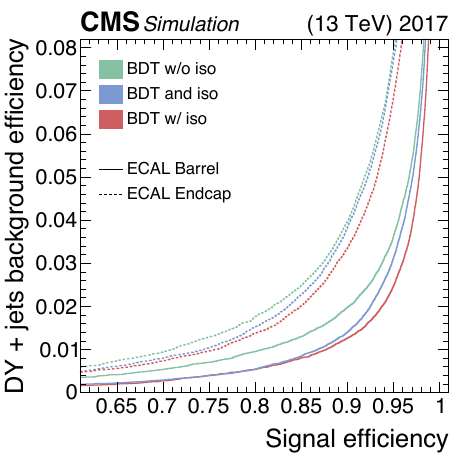
\includegraphics[width=0.5\textwidth]{plots/chapter5/BDT.png}
  \caption{Receiver operating curve showing the background versus signal efficiency for the BDT with and without isolation incorporated in training.}
  \label{fig:elec_BDT}
\end{figure*}

\section{Tau reconstruction}

Hadrons plus strips (HPS) algorithm is used for reconstructing the hadronic decays of tau~\cite{Sirunyan:2018pgf}. ``DeepTau'' based identification is used for discrimination of hadronic decays of tau against jets, electrons, and muons. A detailed description of the HPS algorithm, followed by the DeepTau Identification algorithm, is given in the following subsections.

\subsection{Hadrons Plus Strips}

The HPS algorithm is seeded by jets clustered with the anti-\kt algorithm with a distance parameter $\dr = 0.4$. To reconstruct the energy deposits \Pgpz candidates leave in the ECAL, photon and electron constituents of the jet that seeds the hadronic tau (\tauh) reconstruction are clustered into strips. The \Pe or \Pgg (not yet included in a strip) with the highest \pt is used to build a new strip. The $\eta$ and $\phi$ of this candidate determine the initial position of the strip. The next highest \pt \Pe or \Pgg within an $\eta$--$\phi$ window centered on the strip location is added to the strip. The position is recomputed as the energy-weighted average of the electron/photon constituents in the strip. This procedure is repeated until there are no more electrons or photons with $\pt > 0.5 \GeV$ within the strip window. The $\Delta \eta $ and $\Delta \phi $ of the strip vary based on the \pt or \ET to be added to the strip. It also depends on the energy, the strip already has, as
\begin{linenomath*}
  \begin{equation*}
    \begin{aligned}
      \Delta \eta = f(\pt^{e/\Pgg}) + f(\pt^{\text{strip}}) \\
      \Delta \phi = g(\pt^{e/\Pgg}) + g(\pt^{\text{strip}})
    \end{aligned}
  \end{equation*}
\end{linenomath*}
where $\pt^{e/\gamma}$ is the transverse momentum of the candidate to be added to the strip and $\pt^{\text{strip}}$ is the transverse momentum of the strip before merging a new candidate in. In addition, the strip size is bounded as 0.05 $< \Delta\eta <$ 0.15, 0.05 $< \Delta\phi <$ 0.3. The functions f(\pt) and g(\pt) are defined as
\begin{linenomath*}
  \begin{equation*}
    \begin{aligned}
      f(\pt) = 0.2 \cdot \pt^{-0.66} \\
      g(\pt) = 0.35 \cdot \pt^{-0.71}
    \end{aligned}
  \end{equation*}
\end{linenomath*}

If the $\pt^{\text{strip}}$ is at least 2.5~\GeV, it is considered as a \Pgpz candidate. Hadronic taus are reconstructed by combining charged particles and strips into different signatures compatible with a specific decay mode if the set of cuts listed below is satisfied. If a candidate satisfies more than one of the hypotheses, the one that maximizes the \pt is retained.

The decay modes considered for reconstructing taus are:
\begin{itemize}
  \item One charged particle, no strips.
  \item One charged particle + one strip with mass $0.3 < \mt < 1.3 \cdot \sqrt{\pt/100} \GeV$. The mass window upper limit is constrained to lie between 1.3 and 4.2~\GeV.
  \item Three charged particles with mass $0.8 < \mt < 1.5 \GeV$. The tracks are required to originate within $|\text{dz}| < 0.4$ cm of the same vertex.
  \item Three charged particles and one strip with a total mass $0.8 < \mt < 1.5 \GeV$.
\end{itemize}

The reconstructed hadronic tau candidates are subject to the impact parameter cuts: the impact parameter between the reconstructed hadronic tau and the PV is restricted as $|\text{dz}| < 0.2$ cm to ensure the hadronic tau is associated with the PV.

\subsection{DeepTau}

The application of machine learning techniques has been proven to provide superior results for multi-dimensional problems. DeepTau is a new multiclass tau identification algorithm based on a convolutional deep neural network (DNN). DeepTau combines information from the high-level variables attributed to the reconstructed \tauh candidates with low-level information from the inner tracker, calorimeters, and muon sub-detectors using PF candidates reconstructed within the \tauh signal and isolation cones. DeepTau also takes advantage of using the updated decay mode definitions.

A tau lepton decaying into an electron is referred using \taue, while if it decays into a muon it is referred using \taum, and a jet that is misidentified as a tau lepton is referred with \tauj. A balanced mix of \taue, \taum, \tauh, and \tauj candidates coming from \ttbar, \wjets, and \zjets MC simulation is used to perform the training. The \tauh has a loose preselection: $\pt \in [20, 1000] \GeV$, $\aeta < 2.3$, and $|\text{dz}| < 0.2$, which makes it suitable for the current analysis. The inputs are separated into sets of high-level and low-level features. As high-level inputs, the algorithm takes variables used during tau reconstruction, and one global event variable is the average energy deposition density ($\rho$). For each candidate reconstructed within the tau signal or isolation cones, the 4-momentum, track quality, relation with the PV, calorimeter clusters, and muon stations are used.

The tau signal and isolation cones define two regions of interest in the vicinity of the tau candidate. Based on the angular distance between the reconstructed tau 4-momentum, all available candidates are split into two $\eta \times \phi$ grids of 11 $\times$ 11 (21 $\times$ 21) cells with a cell size of 0.02 $\times$ 0.02 (0.05 $\times$ 0.05) for the signal (isolation) cone. In cases where more than one object of the given type belongs to the same cell, only the object with the highest \pt is considered input. Within each cell, the input variables are split into three blocks: e-gamma, muon, hadrons.

The low-level inputs' organization into two 2D grids allows first processing the local patterns originating from the tau or jet structure. The information obtained is then iteratively combined, covering bigger $\eta \times \phi$ regions up to the point where the total tau signal or isolation cones are covered. The four outputs of the network represent estimates of the reconstructed tau candidate's probabilities to be \taue, \taum, \tauj, or a genuine \tauh. The performance of tau discrimination against quark and gluon induced jets (left), electrons(middle), and muons(right) for DeepTau and the previously available discriminators can be seen in Figure~\ref{fig:deeptau}.

\begin{figure}[hbtp]
  \centering
  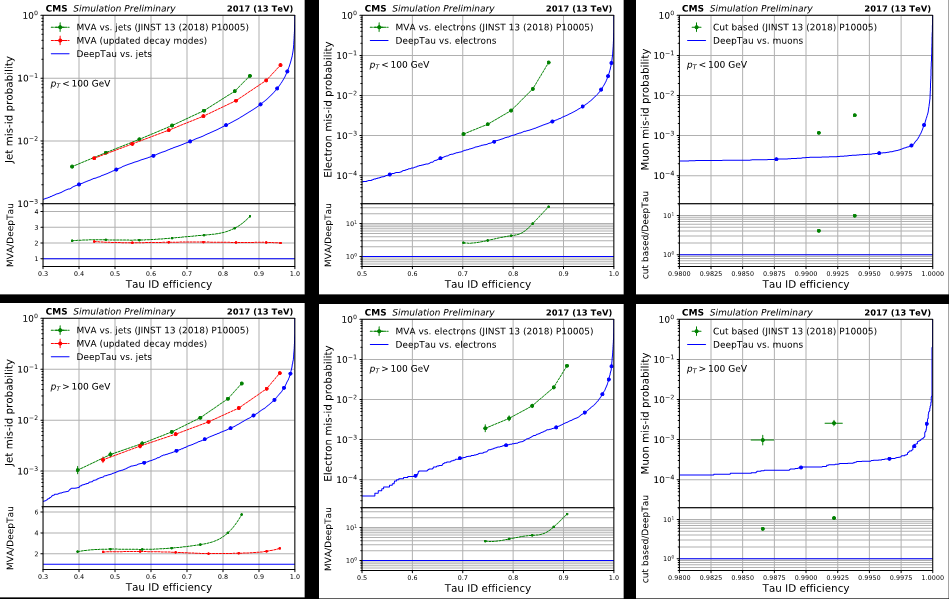
\includegraphics[width=0.98\textwidth]{plots/chapter5/deeptau.png}
  \caption{Performance of tau discrimination against quark and gluon induced jets (left), electrons(middle), and muons(right) for DeepTau and the previously available discriminators.}
  \label{fig:deeptau}
\end{figure}

A WP defined using a \pt dependent threshold on the output of the DNN is used to distinguish \tauh from jets. This WP has a \tauh identification efficiency of about 70\% with a misidentification probability of $\approx 1\%$. This helps to provide a good tau identification efficiency along with high background rejection. The DNN can reject electrons and muons misidentified as \tauh candidates using dedicated criteria based on the consistency between the tracker's measurements, the calorimeters, and the muon detectors. In the \muhad (\ehad) channel, the WP that is used has an efficiency of about 97.5\% (87.5\%) with a misidentification probability of $\approx 1-2\% \, (0.2-0.3\%)$ to discriminate \tauh against electrons, and has an efficiency of about 99.6\% (99.8\%) with a misidentification probability of $\approx 0.04\% \, (0.06\%)$ to discriminate \tauh against muons. DeepTau identification for hadronic taus helps in reducing the Drell-Yan and misidentified lepton background significantly, and the comparison with the previous analysis can be seen in Figure~\ref{fig:collmass}.

\begin{figure}[hbtp]
  \centering
  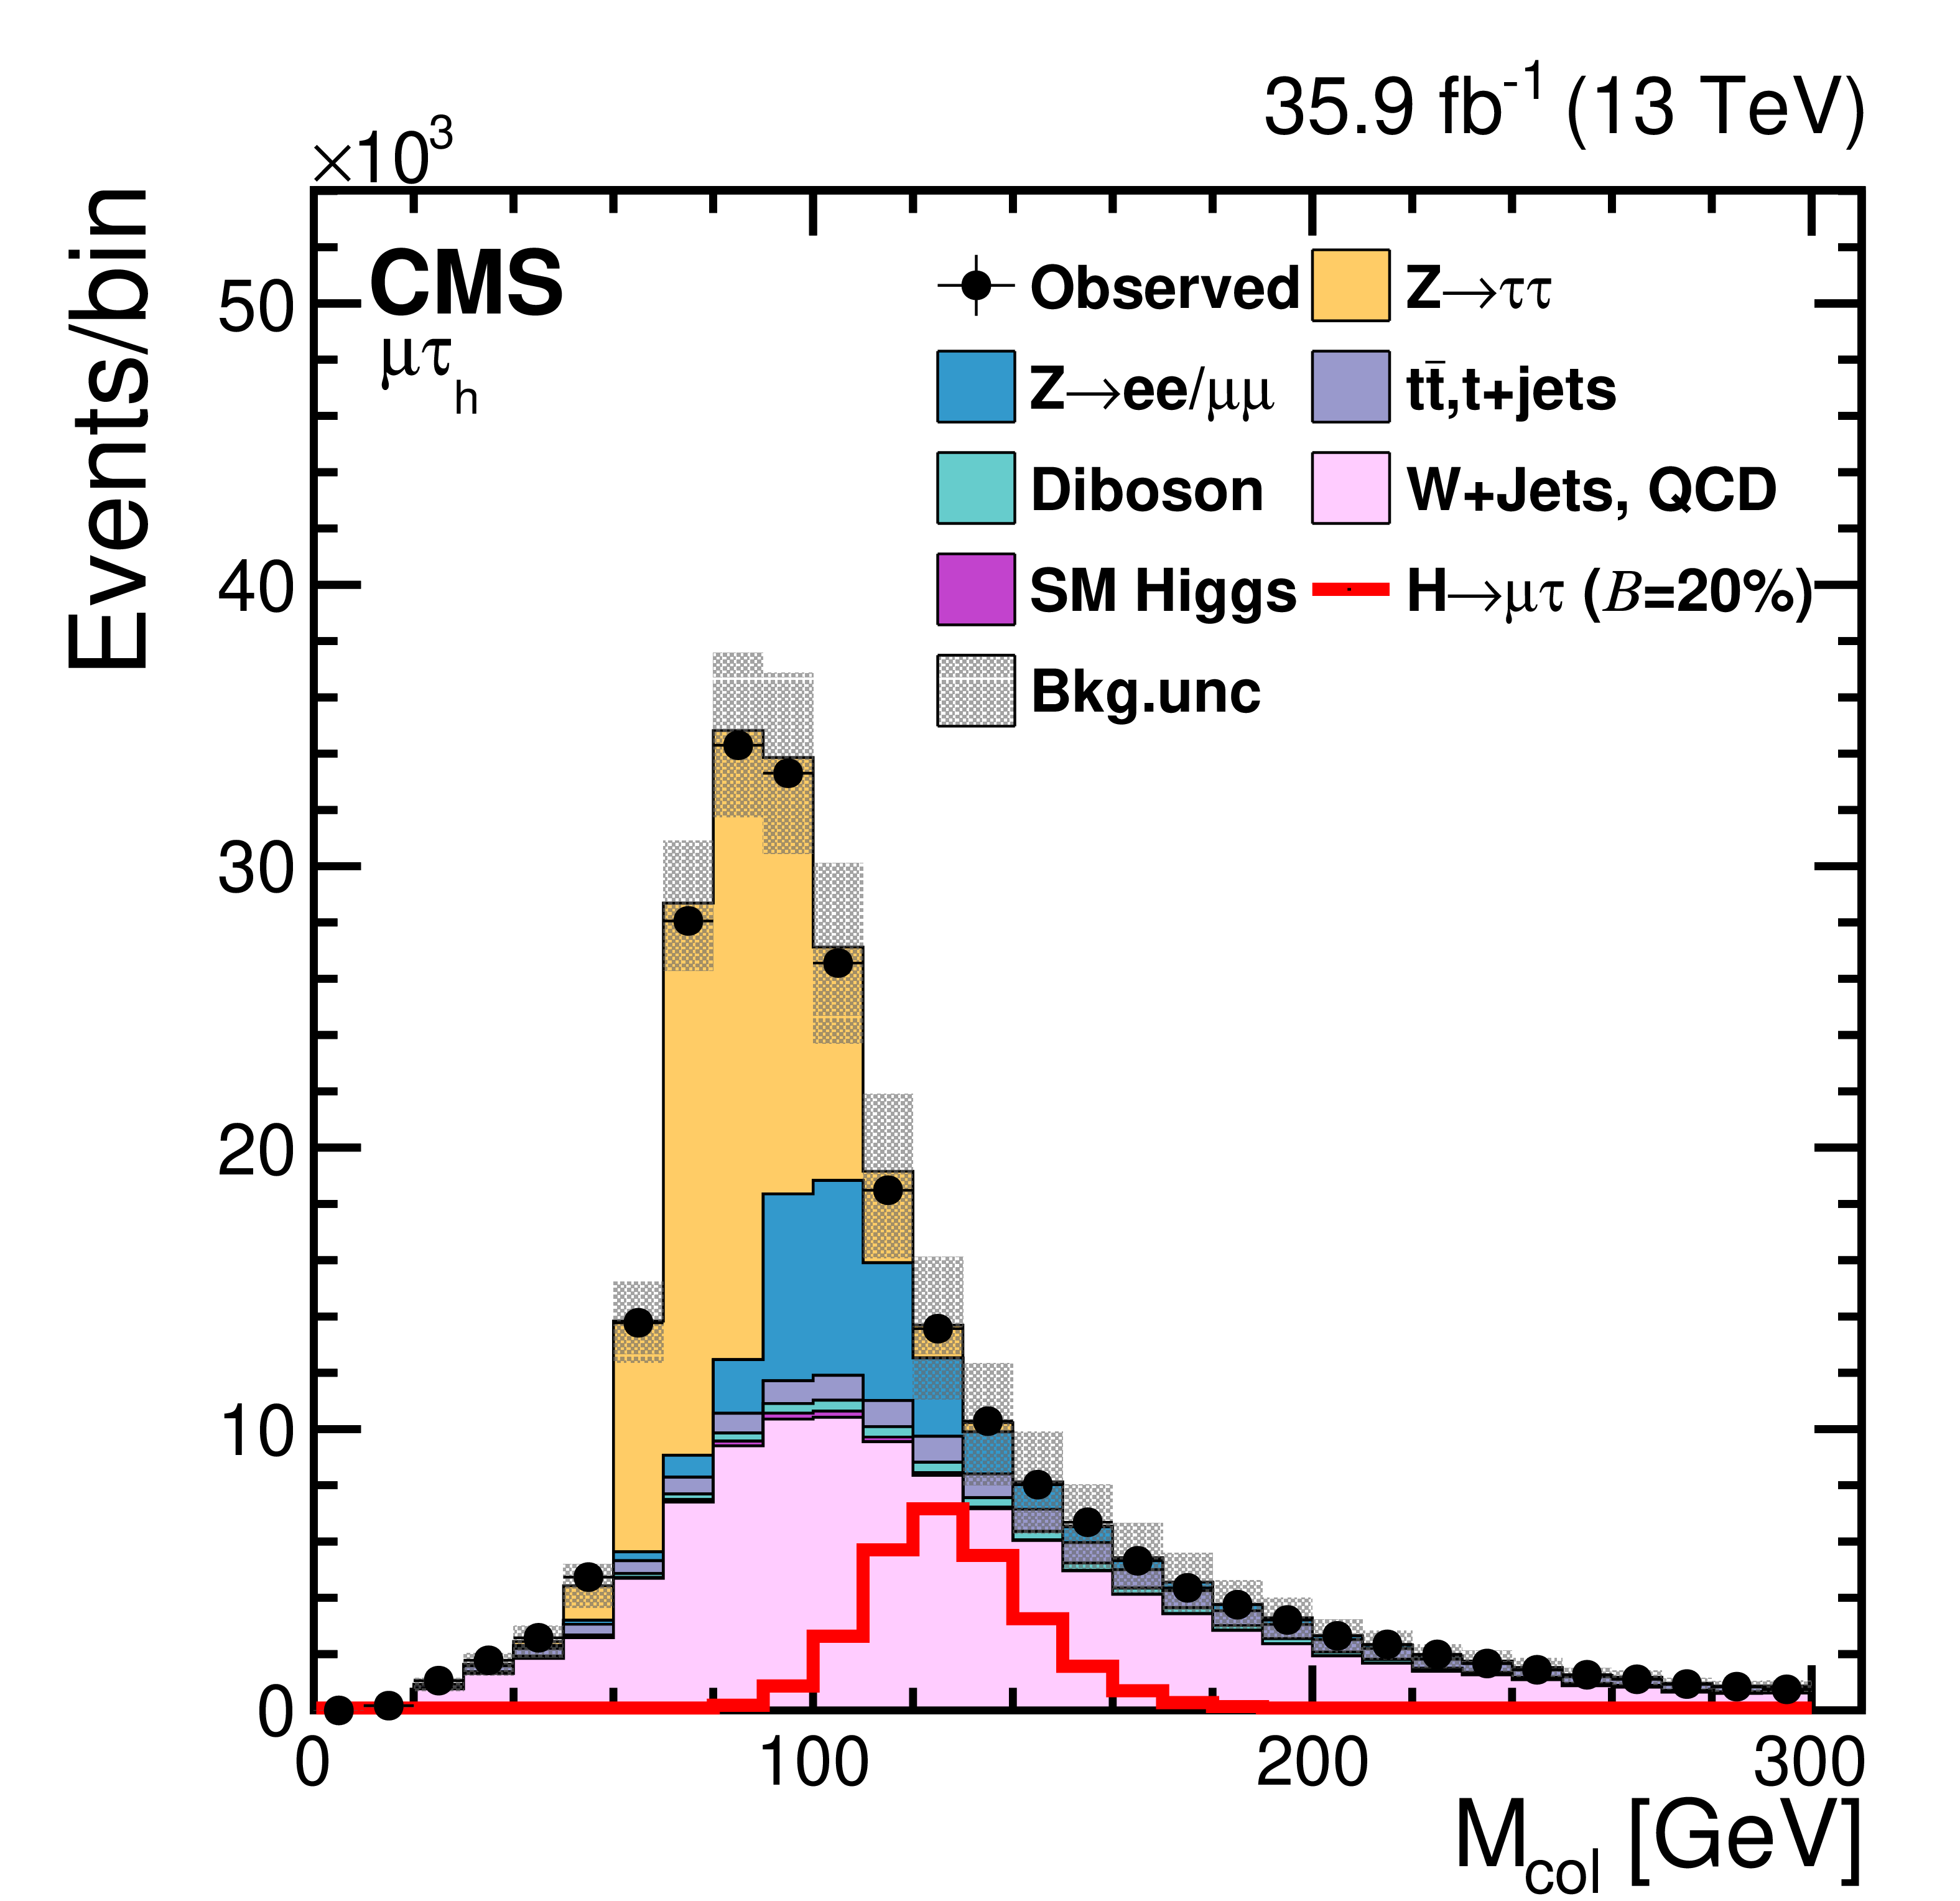
\includegraphics[width=0.49\textwidth]{plots/chapter5/CollMass2016.png}
  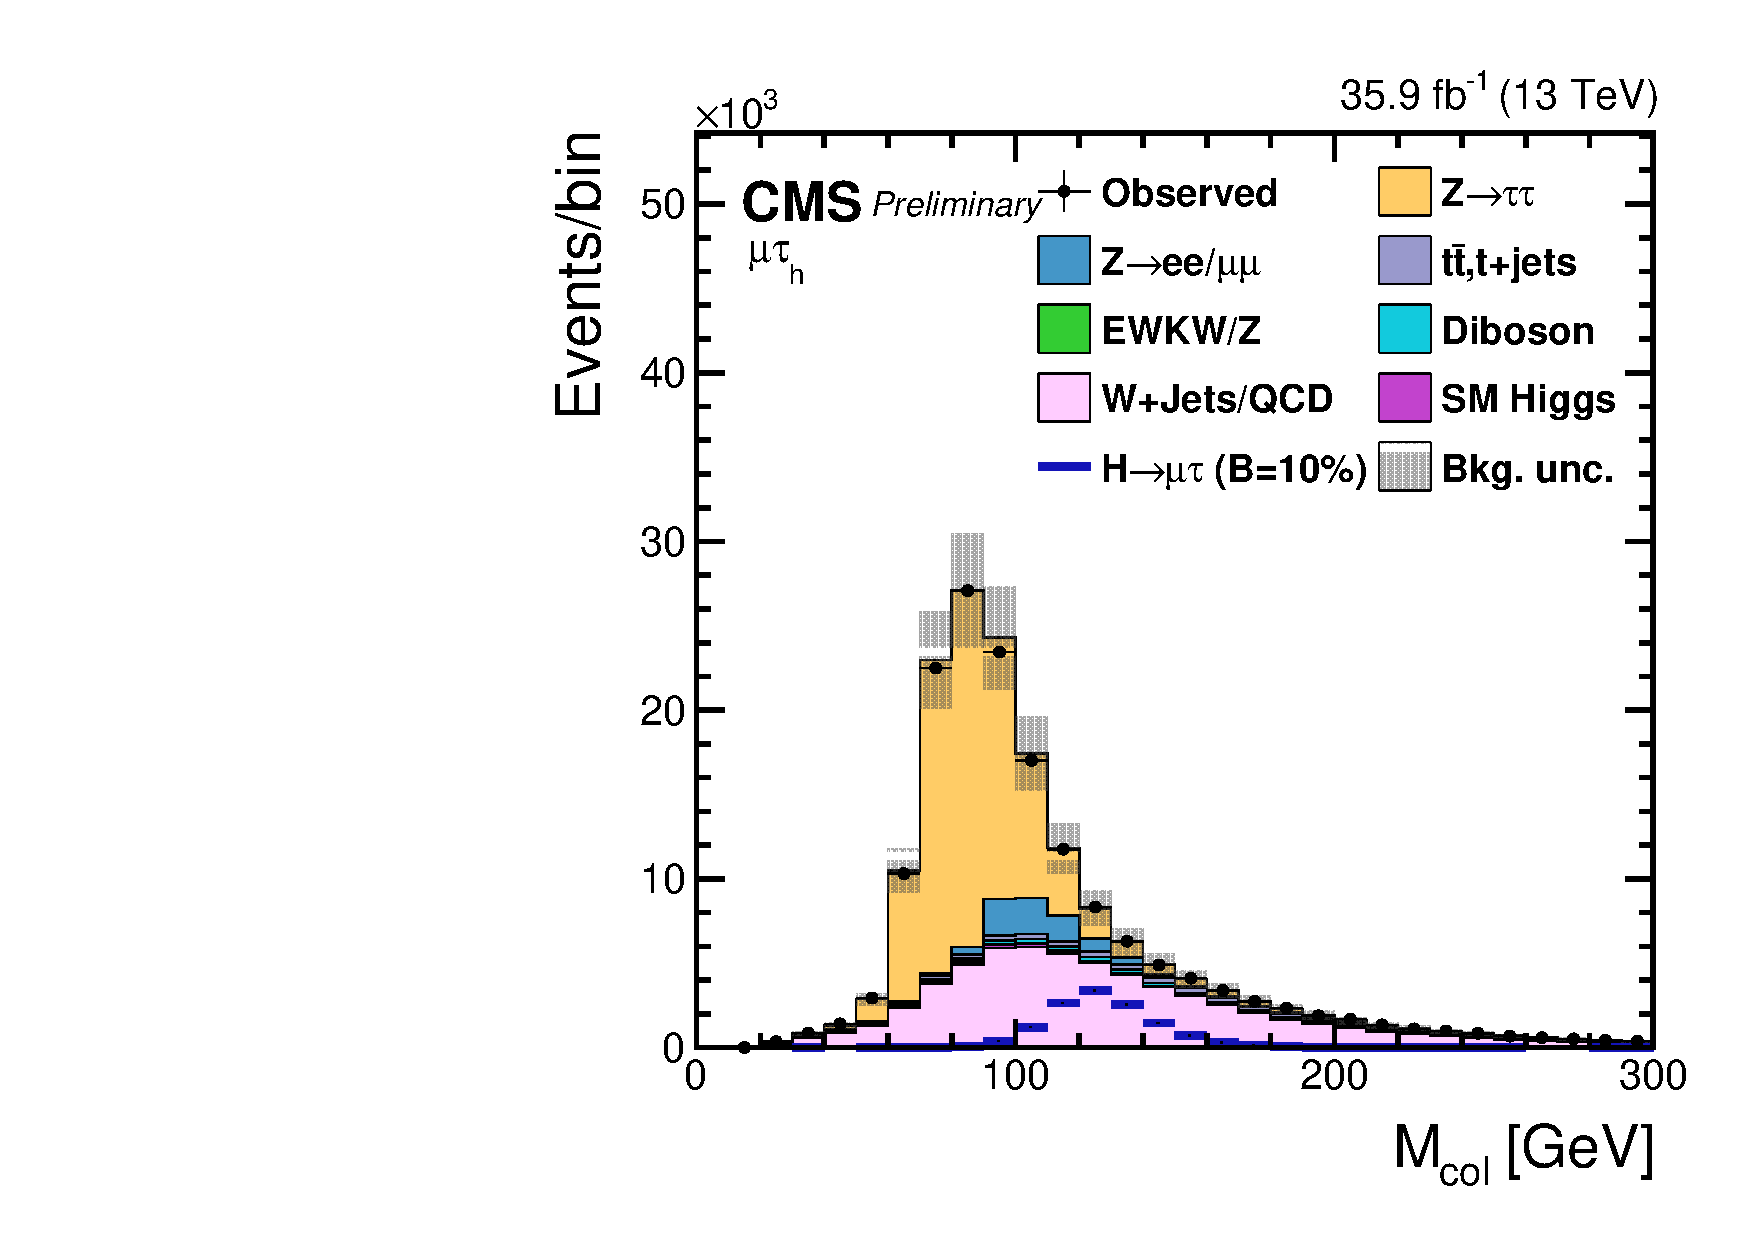
\includegraphics[width=0.49\textwidth]{plots/chapter5/CollMassRun2.pdf}
  \caption{Comparison of the collinear mass distribution from the previous analysis (left) compared to the current analysis (right). As can be seen from the plots, the Drell-Yan background and misidentified lepton background are significantly reduced in the current analysis. This can be attributed to using the DeepTau identification for hadronic taus.}
  \label{fig:collmass}
\end{figure}


\section{Jet reconstruction}

Quarks and gluons hadronize due to color confinement producing a fine spray of particles called jets~\cite{Cacciari:2008gp}. Jets are reconstructed using the anti-\kt clustering algorithm~\cite{Cacciari:2011ma}. This is a sequential clustering algorithm based on the quantities $d_{ij}$, which represents the distance between two entities, and $d_{iB}$, which represents the distance of the i-th object from the beam axis.

These distances are defined as:
\begin{equation}
  \begin{aligned}
  d_{ij}&= \text{min}(k_{ti}^{2p},k_{tj}^{2p})\frac{\Delta_{ij}^{2}}{\text{R}^2} \\
  d_{iB}&=k_{ti}^{2p}
  \end{aligned}
\end{equation}
where $\Delta_{ij}^{2}=(\eta_i-\eta_j)^2+(\phi_i-\phi_j)^2$, $k_{ti}$ is the transverse momentum of the i-th entity and R is the radius parameter which is set as 0.4.

In the anti-\kt clustering algorithm, $p=-1$, where the parameter $p$ governs the relative power of energy versus geometrical scales. The $d_{ij}$ represents the distance between all entity pairs present. If the minimum of those distances is smaller than the minimum distance $d_{iB}$ of any entity from the beam axis, those entities i and j are combined into a single entity. Otherwise, the object closest to the beam axis is considered a jet. It is then removed from the list of entities to be further clustered. The high \pt particles dominate in the anti-\kt and are clustered first. Softer constituents are subsequently clustered. Before the soft particles cluster among themselves, they cluster with hard particles. As a result of this, a hard particle with no hard neighbors within a distance 2R accumulates all the soft particles within a circle of radius R. Anti-\kt tries to produce jets with somewhat conical shapes which are centered around the hardest particles of the event. The boundaries are resilient to the effect of infrared and collinear radiation.

The reconstructed jets' energy differs from their true values as they are complex objects suffering from several effects. Correction factors are applied to calibrate their \pt and ensure a uniform response in $\eta$~\cite{Chatrchyan:2011ds, Khachatryan:2016kdb}. The energy coming from the pileup that has been clustered into the jet needs to be corrected. This is corrected using the hybrid jet area method. This method is a combination of the average offset method and the jet area method. The average amount of energy added to the event due to pileup is measured using the zero bias events in the average offset method. This relies on the assumption that averaging over zero bias events makes this measurement insensitive to high \pt objects. The average offset is measured in bins of $\eta$, and the number of pileup vertices (\npv) averaged over $\phi$. The correction is then given by $1-\frac{<\text{Offset}(\npv,\eta)>}{\pt^{\text{RAW}}}$, where $\pt^{\text{RAW}}$ is the uncorrected jet \pt. The other assumption is that every jet contains the same amount of pileup contribution, which is a drawback for this method.

The jet area method calculates corrections on a jet-by-jet basis. The energy density per event is calculated by clustering jets using the \kt algorithm. The \kt algorithm favors clustering soft jets as opposed to hard ones. The \pt is then divided by jet area, which is defined as the region in $\eta$--$\phi$ occupied by soft particles clustered in the jet. The median of this distribution ($\rho$) for an event is expected to be insensitive to hard particles. This $\rho A_{i}$ is a good approximation of pileup contribution to the i-th jet. However, this approach has a drawback because it doesn't consider the fact that the detector response is $\eta$ dependent. Thus, the hybrid jet area method combines these two methods to calculate a jet-by-jet correction depending on $\eta$ and \npv.

Jet momentum is determined as the vectorial sum of all particle momenta in the jet. It is found from simulation to be, on average, within 5 to 10\% of the true momentum over the whole \pt spectrum within detector acceptance~\cite{CMS:2017wyc}. Data collected in the ECAL endcaps were affected by noise during the 2017 run. This effect is mitigated by discarding events with jets having $\pt < 50 \GeV$ and $2.65 < \aeta < 3.139$ in 2017 dataset. Hadronic jets that contain b quarks are tagged using a DNN called the DeepCSV algorithm, and we use a WP with efficiency $\approx 70\%$~\cite{Sirunyan:2017ezt}.

The energy of reconstructed jets is corrected with an MC calibration factor to match the generated MC particle jet energy on average. The energy response of reconstructed jets is calibrated to be uniform with respect to $\eta$ and \pt. A QCD dijet sample is used to correct the dependence on $\eta$. Using jets that are approximately back-to-back in the azimuthal direction but at different $\eta$ regions of the detector, the difference in response between these two $\eta$ regions can be ascertained and corrected. Using the same method of measuring residual response in the transverse direction in \gjets or \zjets events, the absolute jet energy scale as a function of \pt can be made uniform~\cite{Khachatryan:2016kdb}. Additional selection criteria are applied to each jet to remove jets potentially dominated by instrumental effects or reconstruction failures. When combining information from the entire detector, the jet energy resolution amounts typically to 15\% at 10~\GeV, 8\% at 100~\GeV, and 4\% at 1~\TeV. Any jet within $\Delta\text{R}=0.5$ of the identified leptons is removed.


\section{Missing transverse energy}

Neutrinos and other hypothetical particles that are weakly interacting cannot be detected in the CMS detector. The momentum imbalance in the transverse plane can be used to infer their presence. The missing transverse momentum vector \ptvecmiss is computed as the negative vector sum of all the PF candidates' transverse momenta in an event $\ptvecmiss = -\Sigma\ptvec$, and its magnitude is denoted as \ptmiss~\cite{Sirunyan:2019kia}. The \ptvecmiss is modified to account for corrections to the reconstructed jets' energy scale in the event. Anomalous high-\ptmiss events can be due to various reconstruction failures, detector malfunctions, or non-collision backgrounds. Such events are rejected by event filters designed to identify more than 85--90\% of the spurious high-\ptmiss events with a mistagging rate less than 0.1\%~\cite{Sirunyan:2019kia}. In addition to the event filtering algorithms, the jet identification selection imposed, which requires the neutral hadron energy fraction of a jet to be less than 0.9, rejects more than 99\% of the noisy jets, independent of jet \pt, with a negligible mistag rate.

Corrections to the \ptvecmiss are applied to reduce the mismodeling of the simulated \PZ, \PW, and Higgs boson samples. The corrections are applied to the simulated events based on the vectorial difference of the measured missing transverse momentum and total transverse momentum of neutrinos originating from the decay of the \PZ, \PW, or Higgs boson. Their average effect is the reduction of the \ptmiss obtained from the simulation by a few \GeV. The \ptvecmiss plays a vital role in this analysis as it helps gauge the momentum of the neutrinos from the decaying tau lepton. The \ptvecmiss reconstruction is directly dependent on the reconstruction of all the other objects in the event, from jets to muons to electrons. Consequently, it is sensitive to all the effects that influence these objects' precise reconstruction and calibration.


\section{Relative isolation}
\label{isolation}
The muon (electron) isolation is measured relative to its $\pt^\ell (\ell=\Pe,\Pgm)$, by summing over the \pt of PF particles in a cone with $\Delta R=0.4(0.3)$ around the lepton:
\begin{linenomath*}
  \begin{equation*}
    I^\ell_{\text{rel}} = \left( \sum \pt^{\text{PV\;charged}} + \text{max}\left[0, \sum \pt^{\text{neutral}} + \sum \pt^\Pgg - \pt^{\text{PU}}(\ell)\right]\right) \biggm/ \pt^\ell,
  \end{equation*}
\end{linenomath*}
where $\pt^{\text{PV\;charged}}$, $\pt^\text{neutral}$, and $\pt^{\Pgg}$ indicate the \pt of a charged particle, a neutral particle, and a photon within the cone, respectively. The neutral contribution to isolation from pileup, $\pt^\text{PU}(\ell)$, is estimated from the area of the jet and the median energy density of the event~\cite{Cacciari:2008gn, Cacciari:2007fd} for the electron or from the sum of transverse momenta of charged hadrons not originating from the PV scaled by a factor of 0.5 for the muons. The charged contribution to isolation from the pileup is rejected by requiring the tracks to originate from the PV.
